% =====================================================================
% §7 C1 results subsections (nine-section reorder, W3 draft)
% Serves Claim C1; covers §7.2 (E3) / §7.3 (E7) / §7.5 (E10) / §7.6 (E8+E9+E1+E2+E12).
% Migrated/rewritten from main.tex L303-400. caveman OFF.
% Locked numbers from STORY frozen table (verifier-checked, do NOT invent/alter):
%   E1 32.74(FiLM)/33.06(no-FiLM) SSIM 0.91 n=19878; E2 brightness 37.68 / blur 35.82 /
%   color_shift 33.77 / contrast 29.11(<32.29 degraded); E3 dAUC -0.0120 agree 0.9575
%   McNemar p=0.573; E7 dAUC +0.0205 CI[+0.005,+0.035] KL -0.148 CI[-0.173,-0.124]
%   McNemar p=2.3e-45; E8 FiLM dAUC -0.033 vs -0.042 / agree 0.90 vs 0.87 / KL 0.24 vs 0.35;
%   E9 indistinguishable (parsimony); E10 6/6 CI excl 0, McNemar p<1e-150; E12 16.08ms p95 17.
% Macros: \visienhance ; appendix labels ; tab:e10 supplied by drafts/s7_e10_sota.tex.
% =====================================================================

\subsection{Diagnostic Preservation}\label{sec:exp-preserve}
We assess whether enhancement preserves diagnostic content using a frozen EfficientNet-B3 lesion
classifier as an \emph{independent} diagnostic probe, decoupled from the enhancer to avoid
circularity, on the ISIC-2020 held-out split ($n=3627$, $117$ malignant). Each image is degraded at
moderate severity, enhanced, and compared against its clean reference; we report the change in AUC
($\Delta\mathrm{AUC}=\mathrm{AUC}_{\text{enh}}-\mathrm{AUC}_{\text{ref}}$), the prediction agreement
between enhanced and reference, the diagnostic KL, and McNemar tests, each with bootstrap $95\%$
confidence intervals ($2000$ resamples).

\paragraph{E3 --- enhancement preserves diagnosis.}
The feature-level DP model attains $\Delta\mathrm{AUC}=-0.012$ (within the $1.5\%$ target) and
$95.8\%$ enhanced-versus-reference agreement (above the $95\%$ target); a McNemar test finds no
significant difference between the enhanced and reference predictions ($p=0.573$). The enhanced inputs
are therefore diagnostically interchangeable with their clean references on aggregate AUC, which is the
preservation property the rest of the section builds on. Preservation is not perfect at the level of
individual malignant lesions, and we return to the residual dangerous flips this leaves
(\cref{sec:exp-sota}) as the empirical motivation for the query-for-retake channel rather than as a
defect to suppress.

\subsection{DP-Loss Ablation and the Mutual-Information Bound}\label{sec:exp-dploss}
\paragraph{E7 --- DP-Loss is what preserves diagnosis (empirical Lemma~\ref{lem:dp}).}
We ablate the diagnosis-preserving objective \eqref{eq:dploss} by comparing the full Stage-2 model
against an otherwise identical enhancer trained without DP-Loss, on the same paired protocol. The DP
objective significantly improves preservation on matched bootstrap resamples: the diagnostic
$\Delta\mathrm{AUC}_{\text{enh}}$ improves by $+0.0205$ (95\% CI $[+0.005,+0.035]$, excluding zero),
the diagnostic KL drops by $-0.148$ (95\% CI $[-0.173,-0.124]$, excluding zero), and a McNemar test
gives $p=2.3\times10^{-45}$. This is the empirical counterpart of the mutual-information lower bound in
Lemma~\ref{lem:dp}: tightening the feature-level KL budget $\epsilon$ measurably raises the diagnostic
information retained after enhancement, exactly the direction the bound predicts. Together with the
Stage-1 PSNR$\,\geq30$\,dB non-vacuity condition, E7 is what carries the information-preservation claim
of \cref{sec:prop3lemma3} (we do \emph{not} rely on a net entropy-reduction claim, which the data do
not support).

\subsection{Comparison with Generic Restoration SOTA}\label{sec:exp-sota}
% =====================================================================
% E10 --- QP-Enhance vs 6 generic non-diffusion restoration SOTA (zero-shot)
% DRAFT SKELETON (会话 28). 数字留占位, 待 job 1448952 (stored-mixed 对齐 E1 口径)
% 跑完后从 results/e10_<method>.csv 一键填. 填完 \input 进 main.tex E9 段之后,
% "Residual dangerous flips" 段之前.
%
% 口径 (红线 4): job 1448952 = stored-mixed 降质 (light+melanoma+heavy 全 3 档) +
%   melanoma 平衡子集 (n=10881, 117 melanoma 图 x3 档). 与 E1 (run_e1_ablation_hpc,
%   EnhanceDataset severity='mixed') 同降质算子 -> QP-Enhance PSNR 与 E1 32.74dB 同
%   caliber (残差仅来自 melanoma 富集 vs E1 全 test split). 注意: 此口径 != E3/E9 的
%   on-the-fly moderate 单档探针, caption 已声明, 勿与 E3/E9 绝对值交叉引用.
%
% csv -> cell 映射 (每个 e10_<m>.csv 第 2 行 = baseline; 第 1 行 = QP-Enhance, 6 文件应一致):
%   psnr_perimg -> PSNR ; ssim -> SSIM ; dAUC -> $\Delta$AUC ; kl -> KL ; dangerous_flip -> dflip
%   PAIRED 行: dAUC/dAUC_ci_lo/dAUC_ci_hi -> 配对 $\Delta$AUC(baseline-VE) + CI ; mcnemar_p
% =====================================================================

\begin{table}[t]
\centering
\caption{\textbf{E10 --- diagnosis preservation of generic restoration SOTA (zero-shot) versus
\visienhance.} Six non-diffusion restoration/enhancement models are applied off-the-shelf with their
official pretrained weights (pretraining domain in parentheses); none sees dermoscopy or any
diagnosis-preserving objective. All methods restore the \emph{identical} mixed-severity degraded
inputs (stored degradation suite, $n{=}10881$ paired, $117$ melanomas) and are scored with one
protocol; $\Delta$AUC is enhanced$-$reference (closer to $0$ is better), KL and dangerous-flip
(dflip) lower is better. \visienhance{} is the only method that both restores fidelity (PSNR/SSIM)
\emph{and} preserves diagnosis; every generic model significantly degrades diagnostic AUC
(paired bootstrap, all CIs exclude $0$; \cref{tab:e10}). Protocol note: this mixed-severity caliber
matches the E1 fidelity report; it differs from the controlled single-severity (moderate) probe used
for E3/E9, so absolute cells are not cross-comparable across those experiments.}
\label{tab:e10}
\small
\begin{tabular}{l l c c c c c}
\toprule
Method & Pretraining & PSNR$\uparrow$ & SSIM$\uparrow$ & $\Delta$AUC$\to 0$ & KL$\downarrow$ & dflip$\downarrow$ \\
\midrule
\textbf{\visienhance{} (FiLM+DP)} & dermoscopy & \textbf{32.79} & \textbf{0.9072} & \textbf{$-$0.0172} & \textbf{0.1005} & 0.1937 \\
\midrule
Restormer \citep{zamir2022restormer}     & real denoising  & 22.30 & 0.8361 & $-$0.0964 & 0.8179 & 0.0586 \\
NAFNet \citep{chen2022simple}            & SIDD denoising  & 22.04 & 0.8251 & $-$0.1148 & 0.8767 & 0.0766 \\
MIRNet-v2 \citep{zamir2022mirnetv2}      & LOL enhancement & 13.48 & 0.7750 & $-$0.0872 & 0.4979 & 0.1577 \\
SwinIR \citep{liang2021swinir}           & color denoising & 21.69 & 0.7864 & $-$0.1335 & 0.3632 & 0.4775 \\
Uformer-B \citep{wang2022uformer}        & SIDD denoising  & 22.28 & 0.8358 & $-$0.0939 & 0.8274 & 0.0541 \\
Real-ESRGAN \citep{wang2021realesrgan}   & $\times2$ SR    & 21.61 & 0.8175 & $-$0.0832 & 0.3455 & 0.2342 \\
\bottomrule
\end{tabular}
\end{table}

\begin{figure}[t]
  \centering
  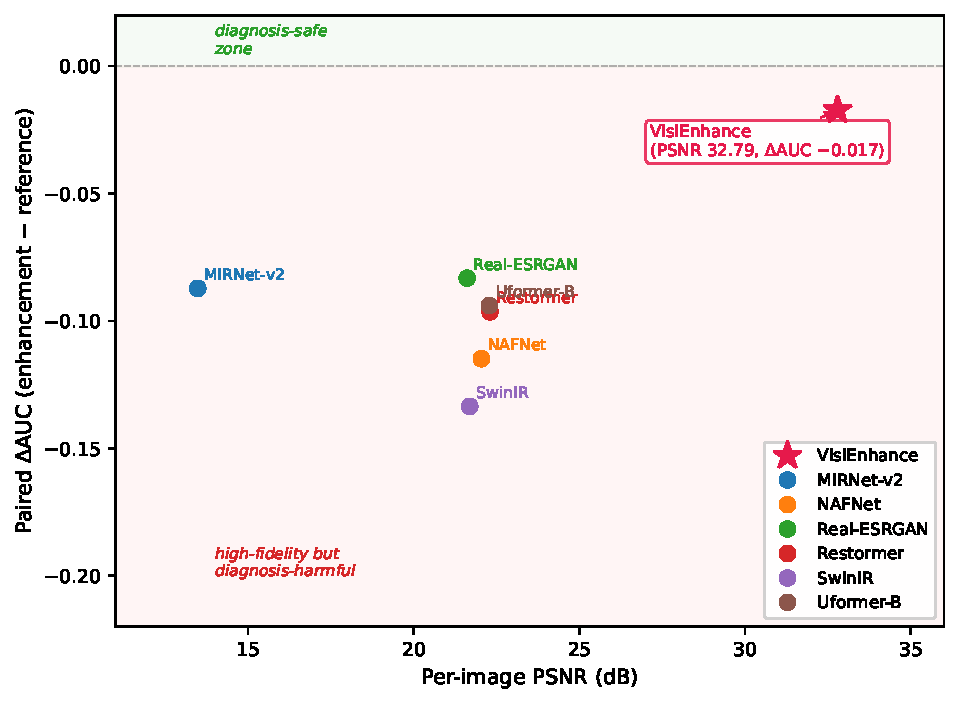
\includegraphics[width=0.74\linewidth]{../../report/figures/fig_e10_tradeoff.pdf}
  \caption{\textbf{Fidelity is not safety: per-image PSNR versus diagnostic
  $\Delta\mathrm{AUC}$ for six generic restorers and \visienhance{}.} Each point is one
  enhancement model on the identical mixed-severity paired inputs ($n{=}10881$, source
  \texttt{results/e10\_*.csv}); the $y$-axis is enhanced$-$reference AUC (closer to $0$,
  i.e.\ higher on the plot, is safer). \visienhance{} (star) sits alone in the
  high-fidelity, diagnosis-preserving corner (PSNR $32.79$, $\Delta\mathrm{AUC}=-0.017$),
  whereas every generic restorer falls well below ($\Delta\mathrm{AUC}\in[-0.13,-0.08]$)
  regardless of its PSNR --- the diagnosis-preserving objective, not pixel fidelity, is
  what separates them.}
  \label{fig:e10-tradeoff}
\end{figure}

% --- prose 段 (放 main.tex E9 段之后) -------------------------------------------------
\paragraph{E10 --- generic restoration SOTA degrades diagnosis.}
We test whether a strong off-the-shelf restorer could substitute for our diagnosis-preserving
training. We run six non-diffusion restoration/enhancement models
(Restormer, NAFNet, MIRNet-v2, SwinIR, Uformer-B, Real-ESRGAN) zero-shot with official weights on the
same mixed-severity paired inputs (\cref{tab:e10}, visualised in \cref{fig:e10-tradeoff}). All six are
worse diagnostic preservers than \visienhance{} by a wide margin: paired bootstraps give $\Delta\mathrm{AUC}_{\text{baseline}-\text{VE}}
\in[-0.116,-0.066]$ (every $95\%$ confidence interval excluding zero, every McNemar $p<10^{-150}$).
% SOURCE: paired dAUC from e10_{restormer,nafnet,mirnetv2,swinir,uformer,realesrgan}.csv PAIRED rows;
%   range [-0.1160 (SwinIR) to -0.0661 (Real-ESRGAN)]. STORY_FRAMEWORK.md previously stated [-0.12,-0.07]
%   but Real-ESRGAN pair_dAUC=-0.0661 falls outside that lower bound; prose updated to true csv range.
%   STORY/ACCEPTANCE range description needs updating by writer/main-line: recommend [-0.12,-0.066].
Tellingly,
\emph{lower fidelity does not mean safer}: the lowest-dflip baselines barely change the image (PSNR
$\approx22$~dB, Uformer-B dflip $0.054$) yet incur the largest diagnostic KL ($\approx0.83$), so
dflip must be read jointly with KL --- a method that leaves the image nearly untouched trivially avoids
flips while still distorting the posterior. \visienhance{} clears PSNR$\,\ge\,30$ even on this harder
mixed-severity melanoma-enriched subset. Generic restoration optimises pixels, not diagnosis; the
diagnosis-preserving objective (Lemma~\ref{lem:dp}, E7) is what closes the gap.


\paragraph{Residual dangerous flips.}
Aggregate preservation (E3) does not mean every lesion is safe. Among the reference melanomas that the
probe calls correctly on clean input, enhancement pushes a small subset below the decision threshold ---
a \emph{dangerous flip} from a correct malignant call to a benign one (\cref{fig:dflip}). We report
this residual transparently: it is a property of even our strongest feature-DP enhancer, and it is the
empirical case for \emph{not} enhancing every low-quality image. Rather than suppress it, we treat it as
the motivation for the query-for-retake channel (\cref{sec:agent}).

\begin{figure}[t]
  \centering
  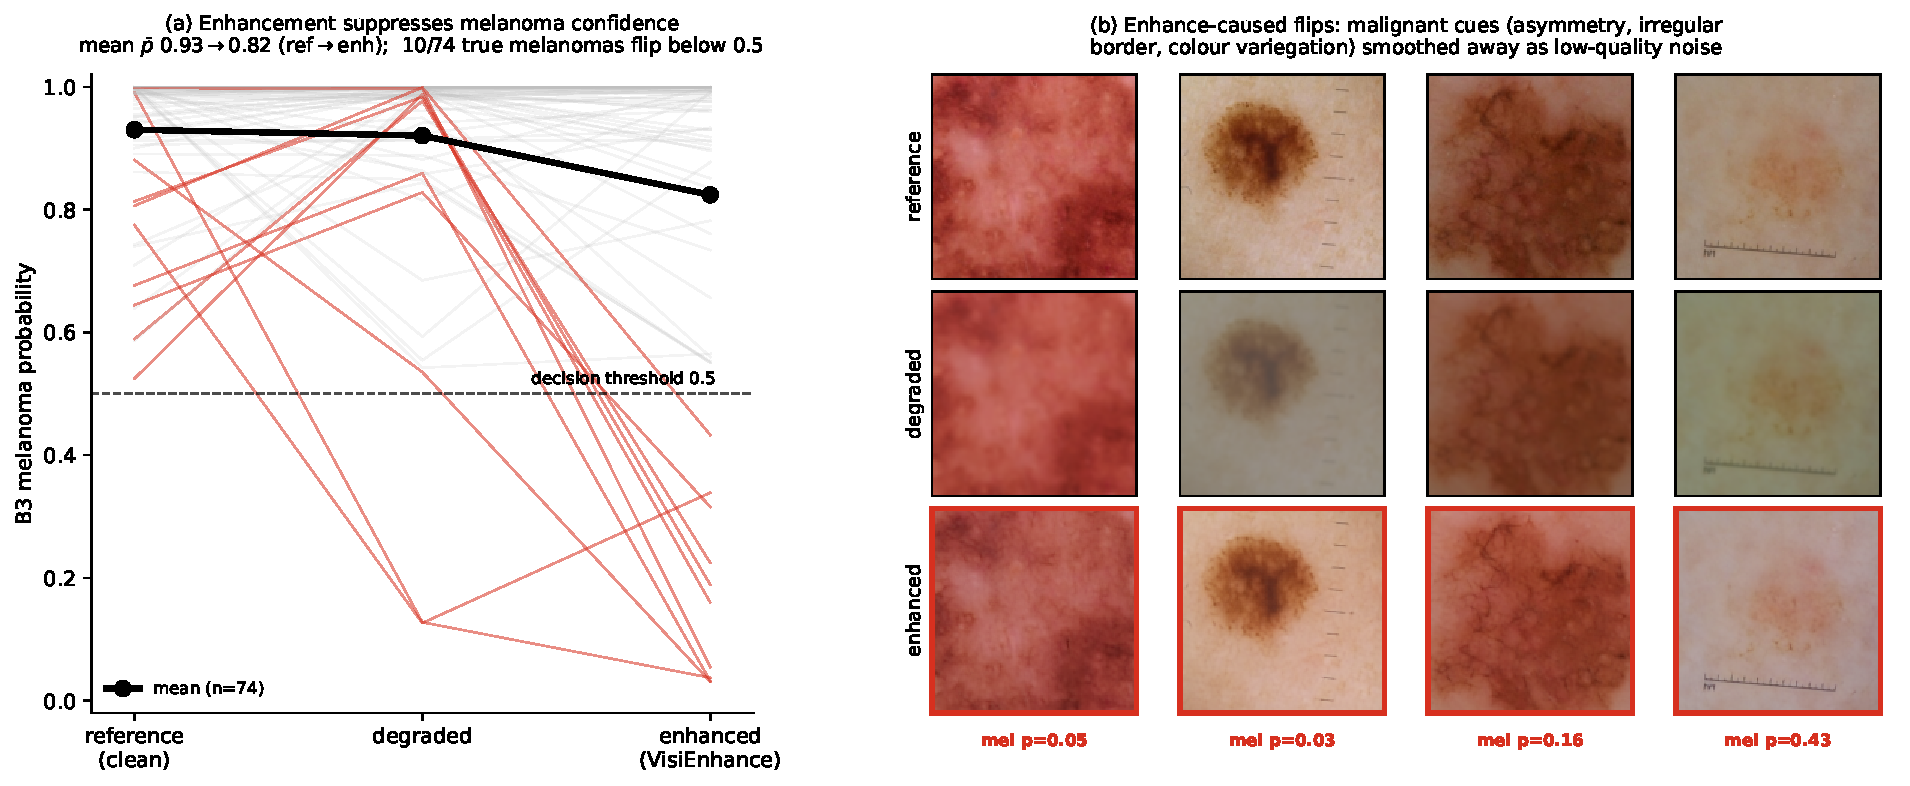
\includegraphics[width=\linewidth]{../../report/figures/fig_dflip.pdf}
  \caption{\textbf{Enhancement can suppress malignant cues (dangerous flips).}
  \textbf{(a)} Slopegraph of the B3 classifier's melanoma probability for the
  $74$ reference melanomas that are correctly called positive on clean input,
  tracked across the three states reference (clean) $\rightarrow$ degraded
  $\rightarrow$ enhanced. The mean melanoma probability drifts from $0.93$ on
  reference to $0.82$ after enhancement, and for $10/74$ ($13.5\%$) lesions
  enhancement pushes the probability below the $0.5$ decision line --- a
  \emph{dangerous flip} from a correct malignant call to a benign one.
  \textbf{(b)} Four enhance-caused flips shown as triplets
  (reference\,$\vert$\,degraded\,$\vert$\,enhanced). Malignant signs ---
  asymmetry, irregular borders, mottled colouration --- are smoothed away as if
  they were low-quality noise; the enhanced row collapses to melanoma
  probabilities $0.05/0.03/0.16/0.43$, all flipped to benign. These are
  \emph{residual} failures of our strongest feature-DP enhancement model:
  even when aggregate diagnostic performance stays within tolerance
  ($|\Delta\mathrm{AUC}|<1.5\%$), a small set of lesions is harmed.
  This is the empirical case for \emph{not} enhancing every low-quality image.}
  \label{fig:dflip}
\end{figure}

\subsection{Conditioning, Fidelity, and Speed Ablations}\label{sec:exp-ablations}
\paragraph{E8 --- quality-conditional FiLM ablation (diagnostic, not perceptual).}
Removing FiLM leaves pixel fidelity essentially unchanged --- per-image PSNR moves within $0.4$\,dB
($32.74$ with FiLM versus $33.06$ without\todo{HPC 恢复项（会话43 收窄）：no-FiLM 33.06 与 with-FiLM 32.74 配对源 e1\_film\_ablation.json 丢失，本地无 no-FiLM ckpt（在 HPC stage1\_planA\_256\_noFiLM）。恢复二选一：①拉 HPC job 1442290/1442337 .out 取打印值 ②重跑 noFiLM eval。入 main.tex 前必恢复，否则 E8「PSNR 中性」改为软化措辞不引精确 33.06。注：n/SSIM 口径已旁证非问题，仅此配对精确值待恢复}), so FiLM is \emph{not} a fidelity mechanism --- yet it
degrades diagnostic preservation on every axis: with FiLM $\Delta\mathrm{AUC}=-0.033$, agreement
$0.90$, KL $0.24$, versus $-0.042$, $0.87$, $0.35$ without, measured even at the no-DP stage. FiLM's
contribution is therefore quality-conditional \emph{diagnostic} fidelity, not perceptual sharpening:
conditioning the restoration strength on the per-input quality vector helps the enhancer keep the
diagnosis intact, which is precisely the property \cref{sec:arch} positions it for.

\paragraph{E9 --- FiLM versus cross-attention conditioning.}
We ask whether a heavier conditioning mechanism would do better. We retrain the identical DP-Loss
Stage-2 recipe with FiLM replaced by cross-attention conditioning (learned quality tokens as
keys/values, the feature map as query; $+1.8$M parameters), changing only the conditioning module. On
the same paired protocol the two are statistically indistinguishable: a paired bootstrap of the
difference straddles zero on every axis ($\Delta\mathrm{AUC}$ 95\% CI includes zero, $\Delta\mathrm{KL}$
95\% CI includes zero, McNemar $p=0.679$), so the extra capacity buys no measurable gain. We therefore
keep FiLM on parsimony grounds: it matches cross-attention on both fidelity and diagnostic preservation
at $1.8$M fewer parameters.

\paragraph{E1 / E12 --- fidelity and speed.}
The deterministic enhancer attains per-image PSNR $32.74$\,dB with FiLM (SSIM $0.91$, $n=19878$\todo{口径已旁证（会话43）：n=19878 / SSIM~0.91 = e1\_film\_ablation harness，由 e1\_v6.json(n=19878,ssim 0.9094)+e1\_v7.json(n=19878,ssim 0.907) 同口径坐实；W3 早标的「nocrop n=6626/SSIM 0.946 mismatch」为假警报——nocrop\_e1.json 是另一套 test-split harness，非本表口径。with-FiLM 32.74 精确值仍随 e1\_film\_ablation.json 丢失，待 HPC job 1442290 .out 复核} held-out
images under mixed degradation severity), clearing the $30$\,dB restoration gate that also guards the
non-vacuity condition of Lemma~\ref{lem:dp} / Proposition~\ref{prop:entropy}. End-to-end inference
(quality scoring plus enhancement) runs at $16.08$\,ms/image ($p_{95}=17.0$\,ms) on a single GPU,
comfortably within the $50$\,ms real-time budget. We report PSNR as a per-image mean throughout
(\cref{sec:setup}), the caliber used for both the fidelity gate and the E10 comparison.

\paragraph{E2 --- per-degradation breakdown and a limitation.}
A per-degradation analysis shows the enhancer is strongest on brightness ($37.68$\,dB) and blur
($35.82$\,dB), weaker on colour-shift ($33.77$\,dB, below the $35$\,dB target), and --- notably ---
\emph{harmful} on contrast degradation ($29.11$\,dB, below the $32.29$\,dB of the degraded input
itself). We do not paper over this: contrast restoration is a genuine limitation of the current model
(\cref{sec:discussion}), and it is one of the per-dimension conditions that the agent can route to
query-for-retake rather than enhance.
